\section{Технический проект}
\subsection{Общая характеристика организации решения задачи}

Необходимо спроектировать и разработать сайт, который должен реализовывать функции онлайн магазина.

Интернет-сайт представляет собой набор взаимосвязанных электронных страниц, которые сгруппированы по разделам, содержащие текстовую, графическую, а также мультимедийную информацию (изображения, видеоролики и пр.). Сайт располагается в Интернете по определенному адресу – доменному имени сайта в виде www.имя\_сайта.ru. Каждая страница web-сайта – это текстовый документ, написанный на языке программирования (HTML, CSS, JavaScript и т.д.).

\subsection{Обоснование выбора технологии проектирования}

На сегодняшний день информационный рынок, поставляющий программные решения в выбранной сфере, предлагает множество продуктов, позволяющих достигнуть поставленной цели – разработки web-сайта.

\subsubsection{Описание используемых технологий и языков программирования}

В процессе разработки web-сайта используются программные средства и языки программирования. Каждое программное средство и каждый язык программирования применяется для круга задач, при решении которых они необходимы.

\subsubsection{Язык программирования Python}

Python – высокоуровневый язык программирования, предназначенный для разработки веб-приложений, а также для написания сценариев и общего программирования. Python широко используется как для создания динамических веб-страниц, так и для разработки разнообразных приложений и систем.

\subsubsection{Язык программирования JavaScript}

\paragraph{Достоинства языка JavaScript}

JavaScript – объектно-ориентированный язык программирования для написания сценариев \cite{javascript}. Чаще всего JavaScript используется для написания сценариев работы с web-страницами, отображаемыми web-браузером. Web-бра\-у\-зер интерпретирует код сценария языка JavaScript, и на основе описанных в сценарии действий производит манипуляции с разметкой web-страницы. Посредством языка JavaScript реализуется возможность программирования на стороне клиента. Предоставляет возможность доступа к элементам разметки web-страницы посредством объектов. При создании сценариев на языке JavaScript приходится сталкиваться с трудностями, связанными с тем, что различные web-браузеры могут по-разному интерпретировать эти сценарии. Серьезные трудности возникают, если какой-либо из браузеров не поддерживает тот или иной объект, метод или свойство. Наиболее практичным способом решения данной проблемы является использование библиотеки jQuery. Данная библиотека реализована на языке JavaScript и расширяет возможности данного языка, нивелируя различия между браузерами.


\subsection{Диаграмма компонентов и схема обмена данными между файлами компонента}

Диаграмма представлений описывает особенности физического представления разрабатываемой системы. Она позволяет определить архитектуру системы, установив зависимости между программными компонентами, в роли которых может выступать как исходный, так и исполняемый код. Основными графическими элементами диаграммы компонентов являются компоненты, интерфейсы, а также зависимости между ними. На рисунке \ref{comp:image} изображена диаграмма компонентов для проектируемой системы. Она включает в себя сервер с операционной системой, на которой установлена система управления содержимым, включающая в себя базу данных и интерфейс. Помимо этого на диаграмме изображен клиентский компьютер с операционной системой, на которой установлен браузер.

\begin{figure}[ht]
\center{\includegraphics[width=1\linewidth]{comp}}
\caption{Диаграмма компонентов}
\label{comp:image}
\end{figure}

Любое представление должно быть вызвано в сценарии страницы web-сайта. Web-страница передает данные.

На рисунке \ref{data:image} представлена схема обмена данными между сценариями представления при вызове представления на странице сайта.

\begin{figure}[ht]
\center{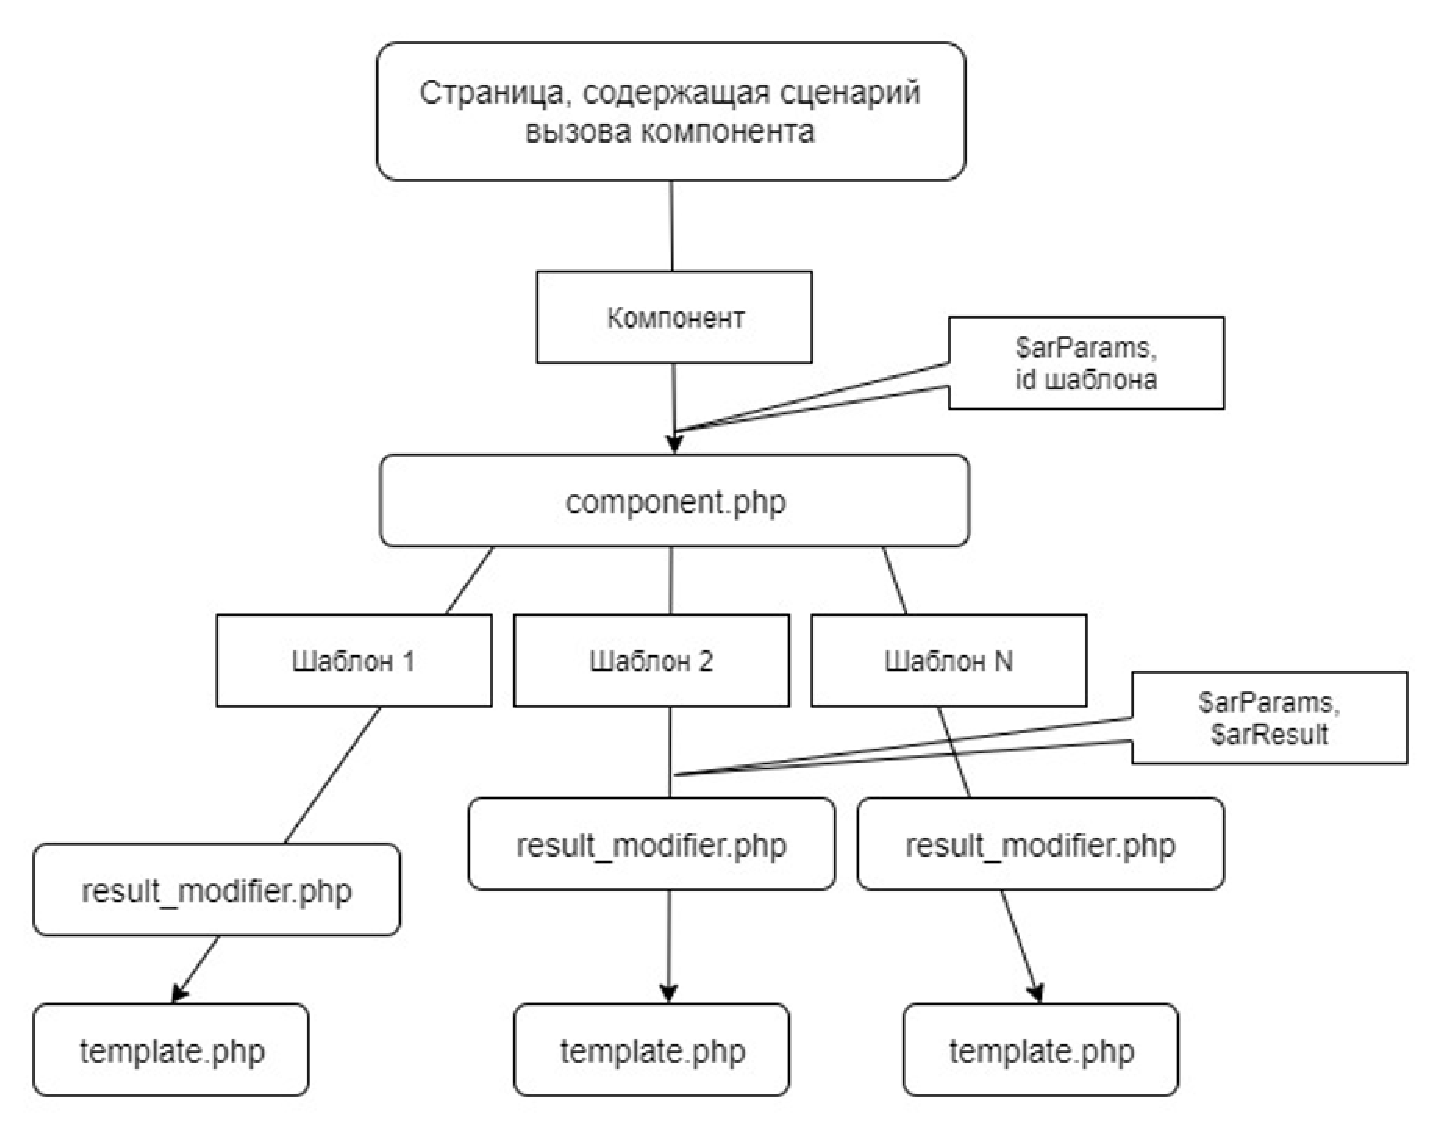
\includegraphics[width=1\linewidth]{data}}
\caption{Диаграмма компонентов}
\label{data:image}
\end{figure}

В файле server.py написан код, который представляет собой простое веб-приложение на Python, использующее фреймворк WSGI (Web Server Gateway Interface).

Здесь импортируются различные библиотеки, классы и функции, которые используются в приложении, такие как CGI, Waitress для веб-сервера, различные представления (views) и функции для работы с файлами и базой данных. Словарь urls соотносит URL-пути с соответствующими представлениями. Когда приходит запрос, код использует этот словарь для определения, какой обработчик использовать для данного URL. Основная функция app обрабатывает POST запрос для загрузки файла, извлекает данные из формы, вставляет изображение в БД и возвращает ответ в формате JSON. Обработка GET запроса происходит с логики определения и вызова соответствующего представления и логики для обработки статических файлов, определение MIME-типа и кодировки для ответа, а также установка заголовков ответа и возврат данных в ответе.

\subsection{Диаграмма размещения}

Диаграмма размещения (рис.~\ref{place:image}) отражает физические взаимосвязи между программными и аппаратными компонентами системы.

\vspace{-8mm} % чтобы убрать пустую строку, которая осталась после переноса рисунка на следующую страницу
\begin{figure}[ht]
\center{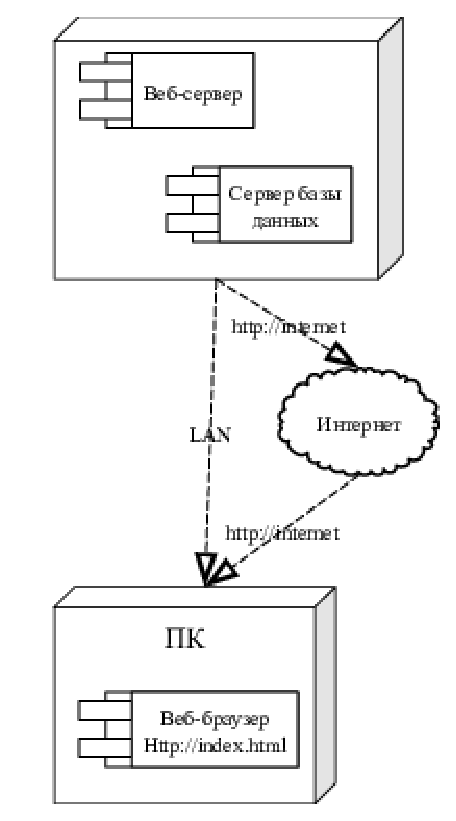
\includegraphics[width=0.57\linewidth]{place}}
\caption{Диаграмма размещения.}
\label{place:image}
\end{figure}



\subsection{Содержание информационных блоков. Основные сущности}

Проанализировав требования, можно выделить две основных сущности:
\begin{itemize}
\item "<Товар">;
\item "<Продукция">;
\end{itemize}

В состав сущности "<Товар"> можно включить атрибуты, представленные в таблице \ref{news:table}.

\begin{xltabular}{\textwidth}{|l|l|p{1.7cm}|X|}
	\caption{Атрибуты сущности "<Товар">\label{news:table}}\\ \hline
	\centrow Поле & \centrow Тип & \centrow Обяза\-тельное & \centrow Описание \\ \hline
	\thead{1} & \thead{2} & \centrow 3 & \centrow 4 \\ \hline
	\endfirsthead
	\continuecaption{Продолжение таблицы \ref{news:table}}
	\thead{1} & \thead{2} & \centrow 3 & \centrow 4 \\ \hline
	\finishhead
	
	\_id & ObjectId & true & Уникальный идентификатор \\ \hline 
	model & String & true & Название модели \\ \hline 
	price & String & true & Цена модели \\ \hline 
	description & TEXT & true & Описание модели \\ \hline 
	count & int & true & Количество доступных пар \\ \hline 
\end{xltabular}


\begin{xltabular}{\textwidth}{|R|C{2.5cm}|l|T|}
	\caption{Атрибуты  сущности "<Заказ">\label{prod:table}}\\ \hline
	\centrow Поле & \centrow Тип & \centrow Обязательное & \centrow Описание \\ \hline
	\centrow 1 & \centrow 2 & \thead{3} & \centrow 4 \\ \hline	
	\_idorder & ObjectId & true & Уникальный идентификатор \\ \hline 
	models & TEXT & true & Модели в заказе \\ \hline 
	totalprice & String & false & Общая сумма заказа \\ \hline 
	count & TEXT & true & Количество пар \\ \hline 
	nameuser & String & false & Имя заказчика \\ \hline 
	adressuser & String & true & Адресс заказчика \\ \hline 
	mailuser & String & true & Электронная почта заказчика \\ \hline 
\end{xltabular}

